% !TeX root = ../../tesis.tex

% -----------------------------------------------------------------------
\subsection{Interconectividad entre Redes}
\label{subsec:interconectividad}
% -----------------------------------------------------------------------

\subsubsection{Integración Multimodal y Conectividad a Nivel de Nodo}
\label{subsubsec:integracion-multimodal}

La interconectividad entre redes es el grado en que distintos modos y líneas de
transporte público ---metro, autobús, trolebús, \brt{}, ciclovías, entre
otros--- operan de manera coordinada como un sistema único y fluido, minimizando
las fricciones de la transferencia y maximizando la cobertura territorial
efectiva del sistema. En la representación por grafos, la interconectividad se
modela introduciendo \termino{aristas de transferencia} que conectan nodos de
diferentes modos o líneas dentro de un mismo grafo multimodal, con pesos que
representan el tiempo de caminata entre andenes, el tiempo de espera esperado y,
en su caso, el costo tarifario adicional del transbordo.

\citet{ugur2025} afirman que la integración juega un papel crucial para
garantizar que los diferentes modos de transporte público operen de manera
armoniosa, facilitando las transferencias y permitiendo a los pasajeros
desplazarse con facilidad entre destinos. En un sistema bien integrado, la
fortaleza de la conexión entre líneas no solo amplía el área accesible para el
usuario, sino que también reduce las dificultades experimentadas durante el
viaje, lo que influye positivamente en la demanda de transporte público y
contribuye a la sustitución del vehículo privado. Su investigación sobre la
línea M7 del metro de Estambul demuestra que la evaluación sistemática de la
conectividad en cada estación ---mediante un
\termino{Índice de Conectividad Simplificado} (\textsc{sci}, por sus siglas en
inglés) que incorpora variables de velocidad, capacidad de pasajeros,
frecuencia, horas de operación y distancia al origen--- revela patrones de
integración desigual que orientan directamente las decisiones de inversión y
mejora operativa.

\subsubsection{Medición de la Conectividad de Parada y Penalización por Transbordo}
\label{subsubsec:penalizacion-transbordo}

La evaluación cuantitativa de la interconectividad requiere un índice que
capture la calidad de la conexión en cada nodo del grafo multimodal, más allá
del simple conteo de líneas que lo sirven. \citet{mishra2015} proponen un marco
de análisis basado en la teoría de grafos que evalúa la conectividad a múltiples
niveles del sistema de transporte: el nivel de nodo (parada individual), el
nivel de línea (ruta) y el nivel de centro de transferencia (
\textit{transfer center}). En este marco, el índice de conectividad de un nodo
se define como el producto de las potencias de conexión de todas las líneas que
lo atraviesan, donde la potencia de conexión de cada línea depende de sus
características operativas ---velocidad, distancia, frecuencia, tiempo de
encabezamiento, capacidad, aceleración y desaceleración--- así como de la
direccionalidad de la ruta.

Este enfoque supera las limitaciones de la centralidad de grado simple, que
únicamente cuenta el número de conexiones directas de un nodo sin considerar la
calidad ni la frecuencia del servicio ofrecido. \citet{mishra2015} subrayan que
medir la conectividad puede resultar una tarea compleja y esquiva, pues es
necesario considerar tarifas, horarios, capacidad, frecuencia y otras
características del sistema en su conjunto; por ello, la evaluación de la
conectividad del transporte requiere un enfoque sistemático que integre los
múltiples parámetros involucrados en la prestación del servicio real. La
diferencia entre un sistema integrado y uno fragmentado se traduce directamente
en la magnitud de la \termino{penalización por transbordo} percibida por el
usuario: cuando la conectividad en los nodos de transferencia es alta, esta
penalización se reduce, haciendo el sistema más atractivo respecto al automóvil
privado.

\subsubsection{El Grafo Multimodal como Marco Formal de Evaluación}
\label{subsubsec:grafo-multimodal}

La representación matemática de la interconectividad entre redes exige la
construcción de un \termino{grafo multimodal} en el que coexistan, sobre una
misma estructura topológica, los nodos y aristas de los distintos modos de
transporte, vinculados mediante aristas artificiales de transferencia
debidamente ponderadas. \citet{mishra2015} señalan que, a diferencia de un
enlace en una red vial ---que es un segmento físico que conecta un nodo con
otro---, un enlace en una red de transporte público multimodal forma parte de
una línea que sirve una secuencia de paradas; dado que diferentes líneas pueden
servir una misma parada, pueden existir múltiples aristas entre los mismos nodos
del grafo, lo que exige representaciones formales más complejas que las de una
red monomodal.

En el modelo computacional implementado en este trabajo, la red de transporte
metropolitana se representa como un grafo dirigido y ponderado
$\grafo = \{\nodos,\, \aristas,\, W\}$, donde $\nodos$ comprende el conjunto de
todas las paradas de todos los modos, $\aristas$ incluye tanto las aristas de
trayecto (intra-línea) como las aristas de transferencia (inter-modo), y $W$ es
la función de peso que asigna a cada arista un costo compuesto ---tiempo de
viaje, tiempo de espera, tiempo de caminata--- calculado a partir de los datos
\gtfs{} de la red. Sobre este grafo unificado, los algoritmos de caminos mínimos
permiten evaluar la interconectividad del sistema de manera integral: una
transferencia deficiente se traduce en un peso elevado en la arista de
transbordo correspondiente, lo que el algoritmo reflejará automáticamente como
una ruta subóptima, señalando así los nodos de transferencia que requieren
intervención prioritaria.

\begin{figure}[H]
  \centering
  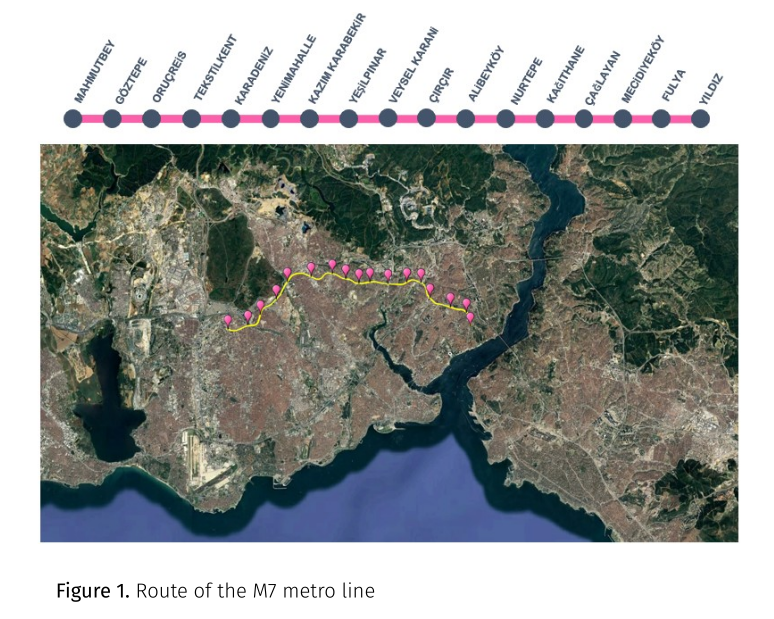
\includegraphics[width=0.88\textwidth]{Figures/Cap3/M7Estambul.png}
  \caption[Índice de Conectividad Simplificado en la línea M7 de Estambul]{
  Distribución del \textsc{sci} a lo largo de las 17 estaciones de la línea M7
  del metro de Estambul (buena, media y débil conectividad).}
  \label{fig:sci-estambul}
  \fuentefigura{\citet{ugur2025}.}
 \end{figure}

La construcción del grafo multimodal $\grafo = \{\nodos,\, \aristas,\, W\}$ que
formaliza esta subsección es el resultado tangible que persigue el Objetivo
Específico 1 (§\ref{subsec:obj-especificos}): sistematizar los datos \gtfs{} de
todos los operadores de la \zmvm{} y unificarlos en una representación
matemática que haga posible el análisis cuantitativo. El Apímetro, descrito en
el \autoref{ch:Capas-codigo}, es la herramienta que ejecuta esta construcción de
forma automatizada y replicable.
